%%%%%%%%%%%%%%%%%%%%%%%%%%%%%%%%%%%%%%%%%%%%%%%%%%%%%%%%%%%%%%%%%%%%%%%
%% $Id: report.tex,v 1.5 2005/02/09 21:06:42 lindstrm Exp $
%%%%%%%%%%%%%%%%%%%%%%%%%%%%%%%%%%%%%%%%%%%%%%%%%%%%%%%%%%%%%%%%%%%%%%%
%% costhesis usage example
%% modified and added to by GQMJr
%%%%%%%%%%%%%%%%%%%%%%%%%%%%%%%%%%%%%%%%%%%%%%%%%%%%%%%%%%%%%%%%%%%%%%%
%
% The costhesis package accepts the following options
%
%   Document types:
%     msc               - Master Thesis
%     bsc		- Kandidate Thesis
%
%   Layout options:
%
%   Other options:
%     blank             - Removes pagenumbers and headers from empty pages
%     blankmsg          - Prints a message of intent on empty pages
%     scheader          - Typeset headers in SMALL CAPS shape (default)
%     slheader          - Typeset headers in slanted shape 
%
%
%
%

\documentclass[12pt,a4paper,twoside,openright]{book}
%%\documentclass[12pt,a4paper,twoside,openright]{memoir}

\usepackage[msc,blankmsg]{costhesis}
%\usepackage[T1]{fontenc}
%%\usepackage{pslatex}
\renewcommand{\rmdefault}{ptm} 
\usepackage{mathptmx}
\usepackage[scaled=.90]{helvet}
\usepackage{courier}
%
\usepackage{bookmark}


%%----------------------------------------------------------------------------
%%   pcap2tex stuff
%%----------------------------------------------------------------------------
 \usepackage[dvipsnames*,svgnames]{xcolor} %% For extended colors
 \usepackage{tikz}
 \usetikzlibrary{arrows,decorations.pathmorphing,backgrounds,fit,positioning,calc,shapes}
% \usepackage{pgfmath}	% --math engine
%%----------------------------------------------------------------------------
%\usepackage[latin1]{inputenc}
\usepackage[utf8]{inputenc} % inputenc allows the user to input accented characters directly from the keyboard
\usepackage[swedish,english]{babel}
\usepackage{rotating}		 %% For text rotating
\usepackage{array}			 %% For table wrapping
\usepackage{graphicx}	 %% Support for images
\usepackage{float}			 %% Suppor for more flexible floating box positioning
\usepackage{color}           %% Support for colour 
\usepackage{mdwlist}
\usepackage{setspace}    %% For fine-grained control over line spacing
\usepackage{listings}		%% For source code listing
\usepackage{bytefield}    %% For packet drawings
\usepackage{tabularx}		%% For simple table stretching
\usepackage{multirow}	%% Support for multirow colums in tables
\usepackage{dcolumn}	%% Support for decimal point alignment in tables
\usepackage{url}	%% Support for breaking URLs
\usepackage[perpage,para,symbol]{footmisc} %% use symbols to ``number'' footnotes and reset which symbol is used first on each page

%%\usepackage{pygmentize}  %% required to use minted -- see python-pygments - Pygments is a Syntax Highlighting Package written in Python
\usepackage{minted}		%% For source code highlighting
\usemintedstyle{borland}

\usepackage{hyperref}		
\usepackage[all]{hypcap}	 %% Prevents an issue related to hyperref and caption linking
%% setup hyperref to use the darkblue color on links
\hypersetup{colorlinks,breaklinks,
            linkcolor=darkblue,urlcolor=darkblue,
            anchorcolor=darkblue,citecolor=darkblue}


%% Some definitions of used colors
\definecolor{darkblue}{rgb}{0.0,0.0,0.3} %% define a color called darkblue
\definecolor{darkred}{rgb}{0.4,0.0,0.0}
\definecolor{red}{rgb}{0.7,0.0,0.0}
\definecolor{lightgrey}{rgb}{0.8,0.8,0.8} 
\definecolor{grey}{rgb}{0.6,0.6,0.6}
\definecolor{darkgrey}{rgb}{0.4,0.4,0.4}
%% Reduce hyphenation as much as possible
\hyphenpenalty=15000 
\tolerance=1000

%% useful redefinitions to use with tables
\newcommand{\rr}{\raggedright} %% raggedright command redefinition
\newcommand{\rl}{\raggedleft} %% raggedleft command redefinition
\newcommand{\tn}{\tabularnewline} %% tabularnewline command redefinition

%% definition of new command for bytefield package
\newcommand{\colorbitbox}[3]{%
	\rlap{\bitbox{#2}{\color{#1}\rule{\width}{\height}}}%
	\bitbox{#2}{#3}}

%% command to ease switching to red color text
\newcommand{\red}{\color{red}}
%%redefinition of paragraph command to insert a breakline after it
\makeatletter
\renewcommand\paragraph{\@startsection{paragraph}{4}{\z@}%
  {-3.25ex\@plus -1ex \@minus -.2ex}%
  {1.5ex \@plus .2ex}%
  {\normalfont\normalsize\bfseries}}
\makeatother

%%redefinition of subparagraph command to insert a breakline after it
\makeatletter
\renewcommand\subparagraph{\@startsection{subparagraph}{5}{\z@}%
  {-3.25ex\@plus -1ex \@minus -.2ex}%
  {1.5ex \@plus .2ex}%
  {\normalfont\normalsize\bfseries}}
\makeatother

\setcounter{tocdepth}{3}	%% 3 depth levels in TOC
\setcounter{secnumdepth}{5} %% 3 sectioning levels. WARNING: command \mainmatter resets this field to its default value!!!
%%%%%%%%%%%%%%%%%%%%%%%%%%%%%%%%%%%%%%%%%%%%%%%%%%%%%%%%%%%%%%%%%%%%
%% End of preamble
%%%%%%%%%%%%%%%%%%%%%%%%%%%%%%%%%%%%%%%%%%%%%%%%%%%%%%%%%%%%%%%%%%%%

\iauthor{My Name}
\ititle{My Report Title}
\isubtitle{My Report Subtitle}
\idate{2012}{January}{21}
\examinername{Professor X}

\setlength{\headheight}{15pt}
\begin{document}

\frontmatter
\selectlanguage{english}
\begin{abstract}
\label{sec:abstract}
\setcounter{page}{1}


Your abstract here.

\end{abstract}
%%\clearpage
\selectlanguage{swedish}
%%\chapter*{Sammanfattning}
\begin{abstract}
\label{sec:swedish_abstract}


IETF xxxx Arbetsgruppen har definierat 
\end{abstract}

\selectlanguage{english}
\begin{acknowledgements}
I would like to acknowldge my adviser's help in getting access to the
necessary packet traffic at a commercial operator (who should be thanked but
must remain unnamed).
\end{acknowledgements}

\selectlanguage{english}
\tableofcontents

\listoffigures

\listoftables

%% add a list of listing if and listings are used
\listoflistings

% \begin{notations}
% \end{notations}

\renewcommand\abbreviationsname{List of Acronyms and Abbreviations}
\begin{abbreviations}
\label{list-of-acronyms-and-abbreviations}

This document requires readers to be familiar with terms and concepts described in \mbox{RFC~1235} \cite{john_ioannidis_coherent_1991}. For clarity we summarize some of these terms and give a short description of them before presenting them in next sections.

\begin{basedescript}{\desclabelstyle{\pushlabel}\desclabelwidth{10em}}
\item[IPv4]					Internet Protocol version 4 (RFC~791 \cite{postel_internet_1981})
\item[IPv6]					Internet Protocol version 6 (RFC~2460 \cite{deering_internet_1998})
\end{basedescript}
\end{abbreviations}

\mainmatter
\setcounter{secnumdepth}{5} 
\chapter{Introduction}
\label{chap:introduction}
%% Longer problem statement
%% General introduction to the area

It was conjectured in \cite{john_ioannidis_coherent_1991} that multicasting
could provide gains by \ldots.

See also \cite{a_new_synchronization_protocol_for_sqlite_databases},
the paper \cite{anand_kannan_n-ary_2012}, 
and the book \cite{brent_s._baxter_standard_1982}.


\section{Problem description}
\label{sec:problem_description}

Page filling text mass. Page filling text mass. Page filling text mass. Page
filling text mass. Page filling text mass. Page filling text mass. Page
filling text mass. Page filling text mass. Page filling text mass. Page
filling text mass. Page filling text mass. Page filling text mass. Page
filling text mass. Page filling text mass. Page filling text mass. Page



\section{Problem context}
\label{sec:problem_context}

Page filling text mass. Page filling text mass. Page filling text mass. Page
filling text mass. Page filling text mass. Page filling text mass. Page
filling text mass. Page filling text mass. Page filling text mass. Page
filling text mass. Page filling text mass. Page filling text mass. Page
filling text mass. Page filling text mass. Page filling text mass. Page


\section{Structure of this thesis}
\label{sec:thesis_structure}

Chapter \ref{chap:introduction} describes the problem and its context.
Chapter \ref{chap:background} provides the background necessary to understand the
problem and the specific knowledge that the reader will need to understand the
rest of this thesis. Following this Chapter \ref{chap:method} describes the
goals, metrics, and solution proposed in this thesis project. The solution is
analyzed and evalued in Chapter \ref{chap:analysis}. Finally, Chapter
\ref{chap:conclusion} offers some conclusions and suggests future work.


\chapter{Background}
\label{chap:background}

%%    What does a reader (another x student -- where x is your study line) need to know to understand your report?
%%    What have others already done?

\section{The Internet Protocol Suite}
\label{sec:the-internet-protocol-suite}

The Internet protocol suite was developed in order to \ldots.

\section{Hardware Abstraction Layer}
\label{sec:hal}

Page filling text mass. Page filling text mass. Page filling text mass. Page
filling text mass. Page filling text mass. Page filling text mass. Page
filling text mass. Page filling text mass. Page filling text mass. Page
filling text mass. Page filling text mass. Page filling text mass. Page
filling text mass. Page filling text mass. Page filling text mass. Page
filling text mass. Page filling text mass. Page filling text mass. Page
filling text mass. The details of the link layer encapsulation will be shown
in Section~\ref{sec:llencap}
Page filling text mass. Page filling text mass. Page filling text mass. Page filling text mass. Page filling text mass. Page filling text mass. Page filling text mass. Page filling text mass. 

\section{Link layer Encapsulation}
\label{sec:llencap}


Page filling text mass. Page filling text mass. Page filling text mass. Page filling text mass. Page filling text mass. Page filling text mass. Page filling text mass. Page filling text mass. Page filling text mass. Page filling text mass. Page filling text mass. Page filling text mass. Page filling text mass. Page filling text mass. Page filling text mass. Page filling text mass. Page filling text mass. Page filling text mass. 

Page filling text mass. Page filling text mass. Page filling text mass. Page
filling text mass. Page filling text mass. Page filling text mass. Page
filling text mass. Page filling text mass. Page filling text mass. Page
filling text mass. Page filling text mass. Page filling text mass. Page
filling text mass. Page filling text mass. Page filling text mass. Page
filling text mass. Page filling text mass.
See Figure~\ref{fig:ieee8023-data-packet} which used the \textsf{bytefield}  \LaTeX\ package. 

%
% Ethernet frame
%
\begin{figure}[h!]
	\centering
\begin{bytefield}{21}
\bitbox[]{7}{} & \bitbox[]{3}{\tiny octets:} & \bitbox[]{4}{\tiny 6} & \bitbox[]{4}{\tiny 6} & \bitbox[]{3}{\tiny 2} & \bitbox[]{5}{\tiny 46 to 1500} & \bitbox[]{3}{\tiny 0 to 46} & \bitbox[]{2}{\tiny 4}\\ 

\bitbox[]{8}{\textbf{ETHERNET \\[-1ex] \tiny{data link-layer}}} & \bitbox[]{2}{} & 

\bitbox{4}{\tiny Destination Address} & \bitbox{4}{\tiny Source Address} & \bitbox{3}{\tiny Length/ Type} & 
\bitbox{5}{\tiny Data Payload} & \bitbox{3}{\tiny Padding} &
\bitbox{2}{\tiny CRC} \\

\bitbox[]{1}{} &\bitbox[]{3}{\tiny octets:} & \bitbox[]{4}{\tiny 7} & \bitbox[]{2}{\tiny 1} & \bitbox[]{0}{$\vdots$ \\[1ex]} & \bitbox[]{16}{} & \bitbox[]{0}{$\vdots$ \\[1ex]} & \bitbox[]{5}{} & \bitbox[]{4}{\tiny Variable}\\

\bitbox[]{4}{\textbf{MAC \\[-1ex] \tiny{packet}}} & \colorbitbox{lightgrey}{4}{\tiny Preamble} & \colorbitbox{lightgrey}{2}{\tiny SFD} & \colorbitbox{lightgrey}{16}{\tiny MAC Client Data} & \colorbitbox{lightgrey}{3}{\tiny Padding} &
\colorbitbox{lightgrey}{2}{\tiny CRC} & \colorbitbox{lightgrey}{4}{\tiny Extension}
\end{bytefield}
     \label{fig:ieee8023-data-packet}
     \caption{Ethernet data link layer protocol encapsulated into a IEEE~802.3 MAC packet}
\end{figure}

Page filling text mass. Page filling text mass. Page filling text mass. Page
filling text mass. Page filling text mass. Page filling text mass. Page
filling text mass. Page filling text mass. Page filling text mass. Page
filling text mass.
See Figure~\ref{fig:pdfexample} was drawn using OpenOffice and output as a PDF
file. 


Page filling text mass. Page filling text mass. Page filling text mass. Page
filling text mass. Page filling text mass. Page filling text mass. Page
filling text mass. Page filling text mass. Page filling text mass. Page
filling text mass. Page filling text mass. Page filling text mass. Page
filling text mass. Page filling text mass. Page filling text mass. Page
Page filling text mass. Page filling text mass. Page filling text mass. Page
filling text mass. Page filling text mass. Page filling text mass. Page
filling text mass. Page filling text mass. Page filling text mass. Page
filling text mass. Page filling text mass. Page filling text mass. Page
filling text mass. Page filling text mass. Page filling text mass. Page
Page filling text mass. Page filling text mass. Page filling text mass. Page
filling text mass. Page filling text mass. Page filling text mass. Page
filling text mass. Page filling text mass. Page filling text mass. Page
filling text mass. Page filling text mass. Page filling text mass. Page
filling text mass. Page filling text mass. Page filling text mass. Page
Page filling text mass. Page filling text mass. Page filling text mass. Page
filling text mass. Page filling text mass. Page filling text mass. Page
filling text mass. Page filling text mass. Page filling text mass. Page
filling text mass. Page filling text mass. Page filling text mass. Page
filling text mass. Page filling text mass. Page filling text mass. Page
Page filling text mass. Page filling text mass. Page filling text mass. Page
filling text mass. Page filling text mass. Page filling text mass. Page
filling text mass. Page filling text mass. Page filling text mass. Page
filling text mass. Page filling text mass. Page filling text mass. Page
filling text mass. Page filling text mass. Page filling text mass. Page
Page filling text mass. Page filling text mass. Page filling text mass. Page
filling text mass. Page filling text mass. Page filling text mass. Page
filling text mass. Page filling text mass. Page filling text mass. Page
filling text mass. Page filling text mass. Page filling text mass. Page
filling text mass. Page filling text mass. Page filling text mass. Page
Page filling text mass. Page filling text mass. Page filling text mass. Page
filling text mass. Page filling text mass. Page filling text mass. Page
filling text mass. Page filling text mass. Page filling text mass. Page
filling text mass. Page filling text mass. Page filling text mass. Page
filling text mass. Page filling text mass. Page filling text mass. Page
Page filling text mass. Page filling text mass. Page filling text mass. Page
filling text mass. Page filling text mass. Page filling text mass. Page
filling text mass. Page filling text mass. Page filling text mass. Page
filling text mass. Page filling text mass. Page filling text mass. Page
filling text mass. Page filling text mass. Page filling text mass. Page

\begin{figure}[h!]
	\centering
%% note that the order for trim is left, bottom, right, and top in lengths
  	\centerline{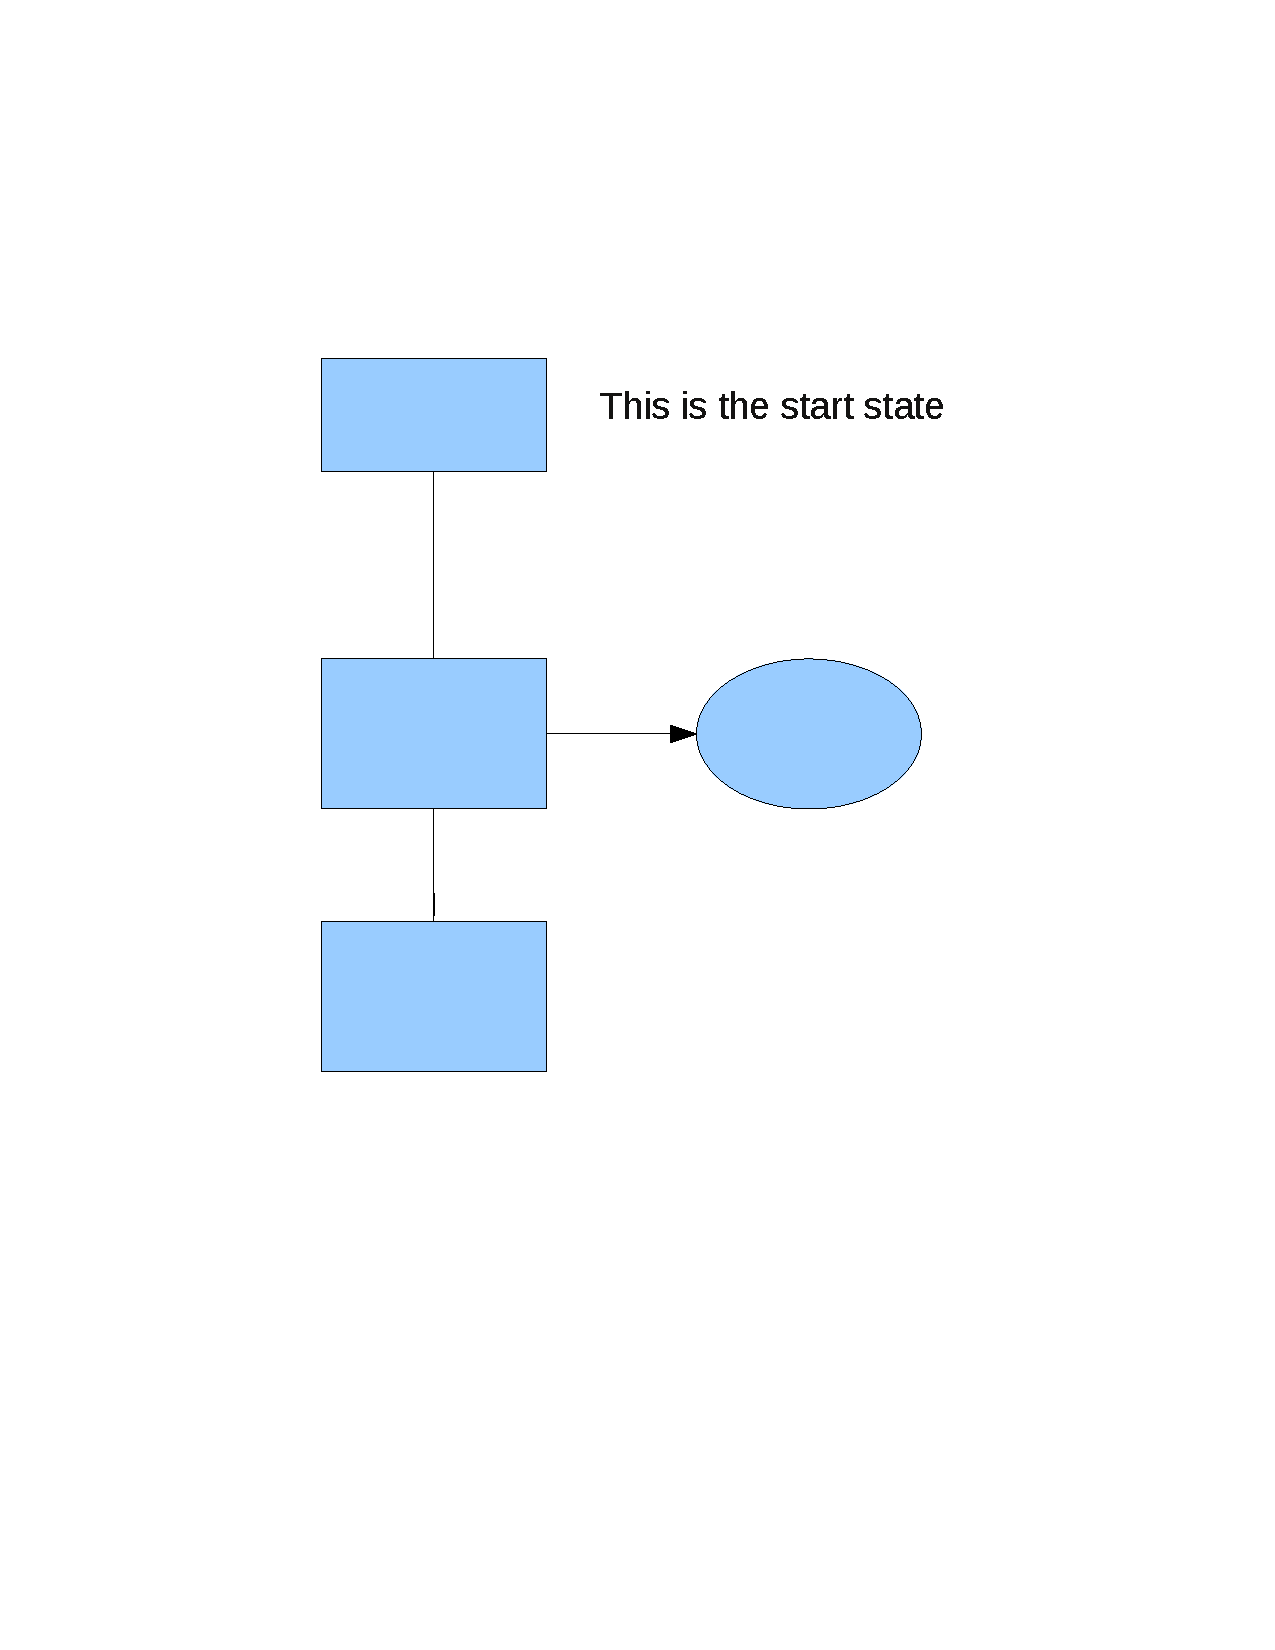
\includegraphics[width=1\textwidth, clip=true, scale=0.5, trim=3cm 9cm 3cm 5cm ]{Random_figure.pdf}}
  	\caption[State diagram from a PDF file.]{This state diagram illustrates nothing in particular.}
  	\label{fig:pdfexample}
\end{figure}


Page filling text mass. Page filling text mass. Page filling text mass. Page
filling text mass. Page filling text mass. Page filling text mass. Page
filling text mass. Page filling text mass. Page filling text mass. Page
filling text mass. Page filling text mass. Page filling text mass. Page
filling text mass.

Page filling text mass. Page filling text mass. Page filling text mass. Page
filling text mass. Page filling text mass. Page filling text mass. Page
filling text mass. Page filling text mass. Page filling text mass. Page
Page filling text mass. Page filling text mass. Page filling text mass. Page
filling text mass. Page filling text mass. Page filling text mass. Page
filling text mass. Page filling text mass. Page filling text mass. Page
filling text mass. Page filling text mass. Page filling text mass. Page
filling text mass. Page filling text mass. Page filling text mass. Page
Page filling text mass. Page filling text mass. Page filling text mass. Page
filling text mass. Page filling text mass. Page filling text mass. Page
filling text mass. Page filling text mass. Page filling text mass. Page
filling text mass. Page filling text mass. Page filling text mass. Page
filling text mass. Page filling text mass. Page filling text mass. Page

The data link layer will receive a packet from the IP layer. The layout of
an IPv4 packet is shown in Figure \ref{fig:ipv4-header}. This should be
contrasted with the IPv6 header shown in \ref{fig:ipv6-header}.

%
% IPv4 packet header
%
\begin{figure}[h!]
	\centering
\begin{bytefield}{32}
\bitheader{0-31} \\
\bitbox{4}{\footnotesize{Version}} & \bitbox{4}{IHL} & \bitbox{6}{\tiny{Type of Service}} & \bitbox{2}{{\scriptsize ECN}} \bitbox{16}{Total Length}\\
\bitbox{16}{Identification} & \bitbox{3}{Flags} & \bitbox{13}{Fragment Offset}\\
\bitbox{8}{Time to Live} & \bitbox{8}{Protocol} & \bitbox{16}{Header Checksum}\\
\wordbox{1}{Source Address}\\
\wordbox{1}{Destination Address}\\
\colorbitbox{lightgrey}{24}{Options} & \colorbitbox{lightgrey}{8}{Padding}
\end{bytefield}
     \label{fig:ipv4-header} 
     \caption[IPv4 datagram header]{IPv4 datagram header. Light grey coloured fields are optional.}
\end{figure}

%
% IPv6 packet header
%
\begin{figure}[h!]
	\centering
\begin{bytefield}{32}
\bitheader{0-31} \\
\bitbox{4}{\footnotesize{Version}} & \bitbox{8}{Traffic Class} & \bitbox{20}{Flow Label}\\
\bitbox{16}{Payload Length} & \bitbox{8}{Next Header} & \bitbox{8}{Hop Limit}\\
\wordbox{4}{Source Address}\\
\wordbox{4}{Destination Address}\\
\end{bytefield}
     \label{fig:ipv6-header}
     \caption{IPv6 datagram header}
\end{figure}

Page filling text mass. Page filling text mass. Page filling text mass. Page
filling text mass. Page filling text mass. Page filling text mass. Page
filling text mass. Page filling text mass. Page filling text mass. Page
filling text mass. Page filling text mass. Page filling text mass. Page
filling text mass. Page filling text mass. Page filling text mass. Page
Page filling text mass. Page filling text mass. Page filling text mass. Page
filling text mass. Page filling text mass. Page filling text mass. Page
filling text mass. Page filling text mass. Page filling text mass. Page
filling text mass. Page filling text mass. Page filling text mass. Page
filling text mass. Page filling text mass. Page filling text mass. Page
Page filling text mass. Page filling text mass. Page filling text mass. Page
filling text mass. Page filling text mass. Page filling text mass. Page
filling text mass. Page filling text mass. Page filling text mass. Page
filling text mass. Page filling text mass. Page filling text mass. Page
filling text mass. Page filling text mass. Page filling text mass. Page
Page filling text mass. Page filling text mass. Page filling text mass. Page
filling text mass. Page filling text mass. Page filling text mass. Page
filling text mass. Page filling text mass. Page filling text mass. Page
filling text mass. Page filling text mass. Page filling text mass. Page
filling text mass. Page filling text mass. Page filling text mass. Page


The code below shows \ldots. While Listing \ref{lst:example} contains an
example of a floating listing.

\begin{samepage}
\begin{minted}[fontsize=\small]{c}
int main() {
  printf("hello, world");
  return 0;
}
\end{minted}
\label{code:foo1}
\end{samepage}

Page filling text mass. Page filling text mass. Page filling text mass. Page
filling text mass. Page filling text mass. Page filling text mass. Page
filling text mass. Page filling text mass. Page filling text mass. Page
filling text mass. Page filling text mass. Page filling text mass. Page
filling text mass. Page filling text mass. Page filling text mass. Page
Page filling text mass. Page filling text mass. Page filling text mass. Page
filling text mass. Page filling text mass. Page filling text mass. Page
filling text mass. Page filling text mass. Page filling text mass. Page
filling text mass. Page filling text mass. Page filling text mass. Page
filling text mass. Page filling text mass. Page filling text mass. Page
Page filling text mass. Page filling text mass. Page filling text mass. Page
filling text mass. Page filling text mass. Page filling text mass. Page
filling text mass. Page filling text mass. Page filling text mass. Page
filling text mass. Page filling text mass. Page filling text mass. Page
filling text mass. Page filling text mass. Page filling text mass. Page
Page filling text mass. Page filling text mass. Page filling text mass. Page
filling text mass. Page filling text mass. Page filling text mass. Page
filling text mass. Page filling text mass. Page filling text mass. Page
filling text mass. Page filling text mass. Page filling text mass. Page
filling text mass. Page filling text mass. Page filling text mass. Page
Page filling text mass. Page filling text mass. Page filling text mass. Page
filling text mass. Page filling text mass. Page filling text mass. Page
filling text mass. Page filling text mass. Page filling text mass. Page
filling text mass. Page filling text mass. Page filling text mass. Page
filling text mass. Page filling text mass. Page filling text mass. Page
Page filling text mass. Page filling text mass. Page filling text mass. Page
filling text mass. Page filling text mass. Page filling text mass. Page
filling text mass. Page filling text mass. Page filling text mass. Page
filling text mass. Page filling text mass. Page filling text mass. Page
filling text mass. Page filling text mass. Page filling text mass. Page
Page filling text mass. Page filling text mass. Page filling text mass. Page
filling text mass. Page filling text mass. Page filling text mass. Page
filling text mass. Page filling text mass. Page filling text mass. Page
filling text mass. Page filling text mass. Page filling text mass. Page
filling text mass. Page filling text mass. Page filling text mass. Page

\lstset{basicstyle=\tiny\ttfamily, tabsize=1, frame=single}

\begin{listing}[H]
\begin{minted}[fontsize=\small]{c}
int main() {
  int scalar = 2;
  int factor = 3;
  int result = scalar * factor

  printf("hello, world with %d", result);
 
  return result;
}
\end{minted}
\caption{Example of a floating listing.}
\label{lst:example}
\end{listing}

Figure \ref{fig:code2} shows two alternative ways of wrting the same
functionality in xxxxxx.

\begin{figure}[h!]
\label{fig:code2}
\begin{minipage}[b]{0.44\linewidth}
\begin{lstlisting}

state : {GREEN, RED}

void semaphore() {
	state = GREEN 	// set initial state
	light(GREEN)
	timer_set(GREEN_TIMER)
	
	while (1) {
		switch(state) {
		case (GREEN): 
			if (timer_expired(GREEN_TIMER)) {
				state = RED
				light(RED)
				timer_set(RED_TIMER)
			}
		case (RED):
			if (timer_expired(RED_TIMER) || 
					pedestrian_button_pressed()) {
				state = GREEN
				light(GREEN)
				timer_set(GREEN_TIMER)
			}
		}
	}
}
\end{lstlisting}
State machine implemented using a traditional loop-switch mechanism.
\end{minipage}
\hspace{0.3cm}
\begin{minipage}[b]{0.52\linewidth}
\begin{lstlisting}

pt_semaphore:
PT_BEGIN
	while (1) {
		light(GREEN)
		timer_set(GREEN_TIMER)
		PT_WAIT_UNTIL(timer_expired(GREEN_TIMER))
		
		light(RED)
		timer_set(RED_TIMER)
		PT_WAIT_UNTIL(timer_expired(RED_TIMER) || 
				pedestrian_button_pressed())
	}
PT_END

\end{lstlisting}
State machine implemented using the protothreads abstraction mechanism.
\end{minipage}
\caption[Code example 1]{Some sample code for example 1.}
\end{figure}

Page filling text mass. Page filling text mass. Page filling text mass. Page
filling text mass. Page filling text mass. Page filling text mass. Page
filling text mass. Page filling text mass. Page filling text mass. Page
filling text mass. Page filling text mass. Page filling text mass. Page
filling text mass. Page filling text mass.  See Table
~\ref{tab:IEEE-802-15-4-phy}.

\begin{table}[h!]
\centering
\caption[Some \mbox{IEEE~802.15.4} physical layers]{Some \mbox{IEEE~802.15.4} physical layers, sorted by release date}\vspace{0.5cm}
\begin{tabularx}{0.93\textwidth}{m{0.15\textwidth} m{0.263\textwidth} m{0.17\textwidth} X }
\small{\textbf{Physical layer (MHz)}} & {\small \textbf{\mbox{Frequency Band} (MHz)}} & {\small \textbf{Modulation} } & {\small \textbf{\mbox{Bit rate} (kb/s)}} \\
\end{tabularx}

\renewcommand\multirowsetup{\rl}

\begin{tabular}{ | r | r m{0.015\textwidth} D{.}{.}{4.1} | m{0.17\textwidth} | r | }
\hline
\multirow{2}{*}{\rl 868/915} 	& 	868 & -- &  868.6 & \multirow{2}{*}{BPSK}  & 20\\
\cline{2-4}
 												& 902 & -- & 928 &  & 40\\
\hline											

\multirow{2}{*}{868/915} 		& 868 & -- & 868.6 & \multirow{2}{*}{ASK} & 250\\
\cline{2-4}
												& 902 & -- & 928 & & 250\\
\hline

\multirow{2}{*}{2,450 (CSS)}	& 	\multirow{2}{*}{2,400}  &	\multirow{2}{0.015\textwidth}{--} & 	\multicolumn{1}{ m{0.115\textwidth} |}{\multirow{2}{*}{ 2,483.5}}	&	\multirow{2}{*}{DQPSK}&	1,000	\\
\cline{6-6}
											& 							&			& &		&	250	\\
\hline

780 											& 779 & -- & 787 			& O-QPSK & 250\\
\hline
\end{tabular}
\label{tab:IEEE-802-15-4-phy}
\end{table}


Page filling text mass. Page filling text mass. Page filling text mass. Page filling text mass. Page filling text mass. Page filling text mass. Page filling text mass. Page filling text mass. Page filling text mass. Page filling text mass. Page filling text mass. Page filling text mass. Page filling text mass. Page filling text mass. Page filling text mass. Page filling text mass. Page filling text mass. Page filling text mass. Page filling text mass. Page filling text mass. Page filling text mass. Page filling text mass. Page filling text mass. Page filling text mass. Page filling text mass. Page filling text mass. Page filling text mass. 

\section{Related work}
\label{sec:related_work}

There are three earlier research projects that have done work related to this
thesis topic. The first considers the problem from the point of view of
throughput as measured in packets per second, the second in terms of
throughput in bits per second, and the third in terms of the number of
messages that are sent per second. Each of these methods will be described in
the following subsections.

\subsection{Packets per second}
\label{ssec:pps}

Page filling text mass. Page filling text mass. Page filling text mass. Page
filling text mass. Page filling text mass. Page filling text mass. Page
filling text mass. Page filling text mass. Page filling text mass. Page
filling text mass. Page filling text mass. 

\subsection{Bits per second}
\label{ssec:bps}

Page filling text mass. Page filling text mass. Page filling text mass. Page
filling text mass. Page filling text mass. Page filling text mass. Page
filling text mass. Page filling text mass. Page filling text mass. Page
filling text mass. Page filling text mass. 

\subsection{Messages per second}
\label{ssec:mps}

Page filling text mass. Page filling text mass. Page filling text mass. Page
filling text mass. Page filling text mass. Page filling text mass. Page
filling text mass. Page filling text mass. Page filling text mass. Page
filling text mass. Page filling text mass. 


\chapter{Method}
\label{chap:method}

%% What are your goals? (What should you be able to do as a result of your solution - which couldn't be done well before you started?)
%%  What you are going to do? Why?

\chapter{Analysis}
\label{chap:analysis}

%% How you are going to evaluate what you have done?
%% Analysis of your data and proposed solution
%% Does this meet the goals which you had when you started?

Figure \ref{fig:processing_vs_payload_length} shows and example of the
performance as measured in your experiments.
Page filling text mass. Page filling text mass. Page filling text mass. Page
filling text mass. Page filling text mass. Page filling text mass. Page
filling text mass. Page filling text mass. Page filling text mass. Page

\begin{figure}[h!]
% GNUPLOT: LaTeX picture
\setlength{\unitlength}{0.240900pt}
\ifx\plotpoint\undefined\newsavebox{\plotpoint}\fi
\begin{picture}(1500,900)(0,0)
\sbox{\plotpoint}{\rule[-0.200pt]{0.400pt}{0.400pt}}%
\put(171.0,131.0){\rule[-0.200pt]{4.818pt}{0.400pt}}
\put(151,131){\makebox(0,0)[r]{ 1.5}}
\put(1419.0,131.0){\rule[-0.200pt]{4.818pt}{0.400pt}}
\put(171.0,212.0){\rule[-0.200pt]{4.818pt}{0.400pt}}
\put(151,212){\makebox(0,0)[r]{ 2}}
\put(1419.0,212.0){\rule[-0.200pt]{4.818pt}{0.400pt}}
\put(171.0,292.0){\rule[-0.200pt]{4.818pt}{0.400pt}}
\put(151,292){\makebox(0,0)[r]{ 2.5}}
\put(1419.0,292.0){\rule[-0.200pt]{4.818pt}{0.400pt}}
\put(171.0,373.0){\rule[-0.200pt]{4.818pt}{0.400pt}}
\put(151,373){\makebox(0,0)[r]{ 3}}
\put(1419.0,373.0){\rule[-0.200pt]{4.818pt}{0.400pt}}
\put(171.0,454.0){\rule[-0.200pt]{4.818pt}{0.400pt}}
\put(151,454){\makebox(0,0)[r]{ 3.5}}
\put(1419.0,454.0){\rule[-0.200pt]{4.818pt}{0.400pt}}
\put(171.0,534.0){\rule[-0.200pt]{4.818pt}{0.400pt}}
\put(151,534){\makebox(0,0)[r]{ 4}}
\put(1419.0,534.0){\rule[-0.200pt]{4.818pt}{0.400pt}}
\put(171.0,615.0){\rule[-0.200pt]{4.818pt}{0.400pt}}
\put(151,615){\makebox(0,0)[r]{ 4.5}}
\put(1419.0,615.0){\rule[-0.200pt]{4.818pt}{0.400pt}}
\put(171.0,695.0){\rule[-0.200pt]{4.818pt}{0.400pt}}
\put(151,695){\makebox(0,0)[r]{ 5}}
\put(1419.0,695.0){\rule[-0.200pt]{4.818pt}{0.400pt}}
\put(171.0,776.0){\rule[-0.200pt]{4.818pt}{0.400pt}}
\put(151,776){\makebox(0,0)[r]{ 5.5}}
\put(1419.0,776.0){\rule[-0.200pt]{4.818pt}{0.400pt}}
\put(171.0,131.0){\rule[-0.200pt]{0.400pt}{4.818pt}}
\put(171,90){\makebox(0,0){ 0}}
\put(171.0,756.0){\rule[-0.200pt]{0.400pt}{4.818pt}}
\put(298.0,131.0){\rule[-0.200pt]{0.400pt}{4.818pt}}
\put(298,90){\makebox(0,0){ 10}}
\put(298.0,756.0){\rule[-0.200pt]{0.400pt}{4.818pt}}
\put(425.0,131.0){\rule[-0.200pt]{0.400pt}{4.818pt}}
\put(425,90){\makebox(0,0){ 20}}
\put(425.0,756.0){\rule[-0.200pt]{0.400pt}{4.818pt}}
\put(551.0,131.0){\rule[-0.200pt]{0.400pt}{4.818pt}}
\put(551,90){\makebox(0,0){ 30}}
\put(551.0,756.0){\rule[-0.200pt]{0.400pt}{4.818pt}}
\put(678.0,131.0){\rule[-0.200pt]{0.400pt}{4.818pt}}
\put(678,90){\makebox(0,0){ 40}}
\put(678.0,756.0){\rule[-0.200pt]{0.400pt}{4.818pt}}
\put(805.0,131.0){\rule[-0.200pt]{0.400pt}{4.818pt}}
\put(805,90){\makebox(0,0){ 50}}
\put(805.0,756.0){\rule[-0.200pt]{0.400pt}{4.818pt}}
\put(932.0,131.0){\rule[-0.200pt]{0.400pt}{4.818pt}}
\put(932,90){\makebox(0,0){ 60}}
\put(932.0,756.0){\rule[-0.200pt]{0.400pt}{4.818pt}}
\put(1059.0,131.0){\rule[-0.200pt]{0.400pt}{4.818pt}}
\put(1059,90){\makebox(0,0){ 70}}
\put(1059.0,756.0){\rule[-0.200pt]{0.400pt}{4.818pt}}
\put(1185.0,131.0){\rule[-0.200pt]{0.400pt}{4.818pt}}
\put(1185,90){\makebox(0,0){ 80}}
\put(1185.0,756.0){\rule[-0.200pt]{0.400pt}{4.818pt}}
\put(1312.0,131.0){\rule[-0.200pt]{0.400pt}{4.818pt}}
\put(1312,90){\makebox(0,0){ 90}}
\put(1312.0,756.0){\rule[-0.200pt]{0.400pt}{4.818pt}}
\put(1439.0,131.0){\rule[-0.200pt]{0.400pt}{4.818pt}}
\put(1439,90){\makebox(0,0){ 100}}
\put(1439.0,756.0){\rule[-0.200pt]{0.400pt}{4.818pt}}
\put(171.0,131.0){\rule[-0.200pt]{0.400pt}{155.380pt}}
\put(171.0,131.0){\rule[-0.200pt]{305.461pt}{0.400pt}}
\put(1439.0,131.0){\rule[-0.200pt]{0.400pt}{155.380pt}}
\put(171.0,776.0){\rule[-0.200pt]{305.461pt}{0.400pt}}
\put(30,453){\rotatebox{-270}{\makebox(0,0){Processing time (ms)}}}
\put(805,29){\makebox(0,0){Payload size (bytes)}}
\put(868.0,131.0){\rule[-0.200pt]{0.400pt}{84.074pt}}
\put(995.0,131.0){\rule[-0.200pt]{0.400pt}{98.287pt}}
\put(1173.0,131.0){\rule[-0.200pt]{0.400pt}{118.041pt}}
\put(1325.0,131.0){\rule[-0.200pt]{0.400pt}{134.904pt}}
\put(1350.0,131.0){\rule[-0.200pt]{0.400pt}{137.795pt}}
\put(1439.0,131.0){\rule[-0.200pt]{0.400pt}{155.380pt}}
\end{picture}
\label{fig:processing_vs_payload_length}
\caption[A GNUplot figure]{Processing time vs. payload length}\vspace{0.5cm}
\end{figure}



Given these measurements, we can calculate our processing bit rate as the inverse of the time it takes to process an additional byte divided by 8 bits per byte:

\[
	bitrate = \frac{1}{\frac{time_{byte}}{8}} = 20.03 \quad kb/s
\] 
 



Page filling text mass. Page filling text mass. Page filling text mass. Page filling text mass. Page filling text mass. Page filling text mass. Page filling text mass. Page filling text mass. Page filling text mass. Page filling text mass. Page filling text mass. Page filling text mass. Page filling text mass. Page filling text mass. Page filling text mass. Page filling text mass. Page filling text mass. Page filling text mass. Page filling text mass. Page filling text mass. Page filling text mass. Page filling text mass. Page filling text mass. Page filling text mass. Page filling text mass. Page filling text mass. Page filling text mass. Page filling text mass. Page filling text mass. Page filling text mass. Page filling text mass. Page filling text mass. Page filling text mass. Page filling text mass. Page filling text mass. Page filling text mass. Page filling text mass. Page filling text mass. Page filling text mass. Page filling text mass. Page filling text mass. Page filling text mass. Page filling text mass. Page filling text mass. Page filling text mass. Page filling text mass. Page filling text mass. Page filling text mass. Page filling text mass. Page filling text mass. Page filling text mass. Page filling text mass. Page filling text mass. Page filling text mass. Page filling text mass. Page filling text mass. Page filling text mass. Page filling text mass. Page filling text mass. Page filling text mass. Page filling text mass. Page filling text mass. Page filling text mass. Page filling text mass. Page filling text mass. Page filling text mass. Page filling text mass. Page filling text mass. 

Table~\ref{tab:main_board} shows part of a table convert from an Excel spreadsheet to a
\LaTeX\ table using Calc2LaTex.

\begin{sidewaystable}\footnotesize
\label{tab:main_board}
\caption{Main board}
\setlength{\leftmargin}{-1cm}
\begin{tabular*}{0.7\textwidth}{|p{2.8cm}|p{6.3cm}|r|r|r|r|r|c|}
\hline
\multicolumn{1}{|c|}{\textbf{PART}} & \multicolumn{1}{c|}{\textbf{TYPE}} & \multicolumn{1}{c|}{\textbf{Digikey part}} & \multicolumn{1}{c|}{\textbf{Order No}} & \multicolumn{1}{c|}{\textbf{Qty}} & \multicolumn{1}{c|}{\textbf{Value}} & \multicolumn{1}{c|}{\textbf{Description}}\\ \hline
B1,B2 & BRIDGE RECTIFIER DF01S & DF01STR-ND & 1470959 & 2 &  &  \\ \hline
C1,C3,C5,C7,C9,\newline
C18,C19,C20,\newline
C21,C22,C23,\newline
C24,C27,C28 & CAPACITOR 0603 (1608 metric) & 399-1095-1-ND & 9406140 & 14 & 100nF &   \\ \hline
C11 & CAPACITOR 0603 (1608 metric) & 445-3454-2-ND & 1710317 & 1 & 470nF &   \\ \hline
C12,C13 & CAPACITOR 0603 (1608 metric) & 445-1270-2-ND & 1740592 & 2 & 12pF &  \\ \hline
C14 & CAPACITOR 0603 (1608 metric) & 445-1289-1-ND & 1740626 & 1 & 470pF &  \\ \hline
C16,C17,C32,C33 & CAPACITOR 0603 (1608 metric) & 445-1272-2-ND & 1740595 & 4 & 18pF &  \\ \hline
C2,C4,C6,C8,\newline
C10,C15 & CAPACITOR 1206 (3216 metric) & 493-2351-1-ND & 1190107 & 6 & 10uF & POL \\ \hline
D1 & DIODE SMAJ58A (DO214A) & SMAJ58ALFTR-ND & 1899460 & 1 &  &  \\ \hline
D2,D3,D5 & DIODE 11DQ09-ND (DO41-10 ) & 11DQ09-ND & 3694069 & 3 &  &   \\ \hline
D4 & DIODE ZENER 60V (SOD123) & MMSZ5264BT1GOSTR-ND & 1895056 & 1 &  & 60V  \\ \hline
JP1,JP2 & CONNECTOR 1x3 MALE &  & 1022249 & 2 &  &  \\ \hline
JP3 & CONNECTOR 2X4 MALE &  & 1022233 & 1 &  &  \\ \hline
JP4 & CONNECTOR 2X7 MALE &  & 1319205 & 1 &  &   \\ \hline
L1 & FERRITE BEAD (1806) & 240-2541-1-ND &  & 1 &  &  \\ \hline
L2 & INDUCTOR 0805 (metric 2012) & 587-2068-1-ND & 1457862 & 1 & 47uH & 160mA  \\ \hline
L3 & INDUCTOR PULSE ENGINEERING\newline
PE53120 & 553-1588-5-ND & 1209561 & 1 & 1000uH &  \\ \hline
L4 & INDUCTOR 0805 (metric 2012) & 587-2046-1-ND & 1457861 & 1 & 22uH &  \\ \hline
LED1 & LED, SMD 1206, RED & 160-1457-1-ND & 1465997 & 1 &  &  \\ \hline
LED2,LED3 & LED, SMD 1206, GREEN & 160-1456-1-ND & 1466000 & 2 &  &  \\ \hline
LED4 & LED, SMD 1206, YELLOW & 160-1458-1-ND & 1465998 & 1 &  &  \\ \hline
Q1 & CRYSTAL 32,768 kHz (TC26H) & 300-8303-ND & 1457084 & 1 &  &  \\ \hline
Q2 & CRYSTAL 32MHz (HC49/US) & 300-8518-ND & 1078935 & 1 &  &  \\ \hline
Q3 & CRYSTAL 25MHz (HC49/US) & 300-8513-ND & 2057969 & 1 &  &  \\ \hline
R1,R13,R15 & RESISTOR 0603 & RMCF0603FT47K0CT-ND & 1469811 & 3 & 47k &  \\ \hline
R10,R11 & RESISTOR 0603 & P330HCT-ND & 1469803 & 2 & 330 &   \\ \hline
R12,R14 & RESISTOR 0603 & RMCF0603FT10K0CT-ND & 1469748 & 3 & 10k &  \\ \hline
R2,R3,R8 & RESISTOR 0603 & P470HCT-ND & 1469815 & 3 & 470 &  \\ \hline
RBIAS & RESISTOR 0603 & P2.32KHTR-ND & 1170823 & 1 & 2.32k &  \\ \hline
RCLASS & RESISTOR 0805 & P953CTR-ND & 1653044 & 1 & 953 &  \\ \hline
RDET & RESISTOR 0603 & P24.9KHTR-ND & 1469785 & 1 & 24.9k &  \\ \hline
RLIM & RESISTOR 0603 & P442KHTR-ND & 1171050 & 1 & 442k &  \\ \hline
RPULLUP & RESISTOR 0603 & P24KGTR-ND & 1469784 & 1 & 24k &  \\ \hline
S1, S2 & PUSH BUTTONS DTSM6 & 679-2383-2-ND &  & 2 &  &   \\ \hline
T1 & RJ45 JACK 7499211123 & 732-1862-ND &  & 1 &  &  \\ \hline
U1 & MSP430F5437a & MSP430F5437AIPN-ND & \multicolumn{1}{l|}{} & 1 &  &  \\ \hline
U2 & ENC28J60 & ENC28J60-I/ML-ND & 1564400 & 1 &  &  \\ \hline
U3 & TPS2375 & 296-17061-ND & 8456860 & 1 &  &   \\ \hline
X1 & CONNECTOR DC INPUT &  & 1243245 & 1 &  &   \\ \hline
\end{tabular*}
\end{sidewaystable}

Page filling text mass. Page filling text mass. Page filling text mass. Page filling text mass. Page filling text mass. Page filling text mass. Page filling text mass. Page filling text mass. Page filling text mass. Page filling text mass. Page filling text mass. Page filling text mass. Page filling text mass. Page filling text mass. Page filling text mass. Page filling text mass. Page filling text mass. Page filling text mass. Page filling text mass. Page filling text mass. Page filling text mass. Page filling text mass.

\chapter{Conclusions}
\label{chap:conclusion}

This chapter explains the conclusions obtained throughout the design,
development, and evaluation described in this thesis and proposes a number of
improvements, extensions, or complements that may be of interest in order to
continue this work. Page filling text mass. Page filling text mass. Page
filling text mass. Page filling text mass. Page filling text mass. Page
filling text mass. Page filling text mass. Page filling text mass. Page
filling text mass. Page filling text mass. Page filling text mass.

\section{Conclusion}
%% Did you meet your goals?
%% What insights have you gained?
%% What suggestions can you give to others working in this area?
%% If you had it to do again, what would you have done differently?


In this section we will state the conclusions and insights gained as result of this thesis project.

\subsection{Goals}
\label{ssec:goals}

The project met five of the ten initial goals. With the third goal not
addressed at all and goals 6-10 only partially met. Page filling text
mass. Page filling text mass. Page filling text mass. Page filling text
mass. Page filling text mass. Page filling text mass. Page filling text
mass. Page filling text mass. Page filling text mass. Page filling text
mass. Page filling text mass.


\subsection{Insights and suggestions for further work}
\label{ssec:insights-and-suggestions}

One of the most important insights to come from this work is the need to
understand the interaction between the IP layer and the link
layer. Unforunately I did not have time to examine this in detail in this
thesis. However, the data shows that paying attendtion to this APR cache
flushing patterns could yield improved performance. Future works should start
by measuring the relationship between the cache validity and number of packets
which are generated at or above the IP layer, but not transmitted on the
network.  Page filling text mass. Page filling text mass. Page filling text
mass. Page filling text mass. Page filling text mass. Page filling text
mass. Page filling text mass. Page filling text mass. Page filling text
mass. Page filling text mass. Page filling text mass.

\section{Future work}
\label{sec:future-work}
%% What you have left undone?
%% What are the next obvious things to be done?
%% What hints can you give to the next person who is going to followup upon your work?


Due to the breadth of the problem, only some of the initial goals have been
met. In these section we will focus on some of the remaining issues that
should be addressed in future work. Page filling text mass. Page filling text
mass. Page filling text mass. Page filling text mass. Page filling text
mass. Page filling text mass. Page filling text mass. Page filling text
mass. Page filling text mass. Page filling text mass. Page filling text mass.

\subsection{What has been left undone?}
\label{what-has-been-left-undone}

The prototype does not address the third requirment, i.e., a yearly
unavailability of less than 3 minutes, this remains an open problem.  Page
filling text mass. Page filling text mass. Page filling text mass. Page
filling text mass. Page filling text mass. Page filling text mass. Page
filling text mass. Page filling text mass. Page filling text mass. Page
filling text mass. Page filling text mass.

\subsubsection{Cost analysis}

The current prototype works, but the performance from a cost perspective makes
this an impractical solution. Future work must reduce the cost of this
solution, to do so a cost analysis needs to first be done. Page filling text
mass. Page filling text mass. Page filling text mass. Page filling text
mass. Page filling text mass. Page filling text mass. Page filling text
mass. Page filling text mass. Page filling text mass. Page filling text
mass. Page filling text mass.

\subsubsection{Security}

A future research effort is needed to address the security holes that results
from using a self-signed certificate. Page filling text mass. Page filling
text mass. Page filling text mass. Page filling text mass. Page filling text
mass. Page filling text mass. Page filling text mass. Page filling text
mass. Page filling text mass. Page filling text mass. Page filling text mass.


\subsection{Next obvious things to be done}

In particular, the author of this thesis wishes to point out xxxxxx remains as
a problem to be solved. Solving this problem is the next thing that should be
done. Page filling text mass. Page filling text mass. Page filling text
mass. Page filling text mass. Page filling text mass. Page filling text
mass. Page filling text mass. Page filling text mass. Page filling text
mass. Page filling text mass. Page filling text mass.

\section{Required Reflections}
\label{sec:req-reflections}


\bibliography{report}
%%\bibliographystyle{IEEEtran}
%%\bibliographystyle{unsrturl}
%%\bibliographystyle{unsrtnat}
\bibliographystyle{myIEEEtran}
\appendix
\chapter{Insensible Approximation}

\backmatter

\end{document}
